\section{Answers arrive in a step}
\label{sec:step}

Figure~\ref{fig:read}a shows how often the answer a model gives can be read from where its state is, layer by layer, for held-out questions. In every model the curve has the same shape: a low plateau, a jump within a few layers, and a high plateau. In Llama-3.1-8B readability rises from below 30\% to 71\% between layers 13 and 15 and reaches \PeakLlama{}; in Qwen2.5-7B the jump comes later, at layer \OnsetLayerQwen{} of 28, and reaches \PeakQwen{}. The depth of the jump differs between models (Table~\ref{tab:models}) but in each it is a sharp event, not a slow approach.

\begin{figure*}[t]
\centering
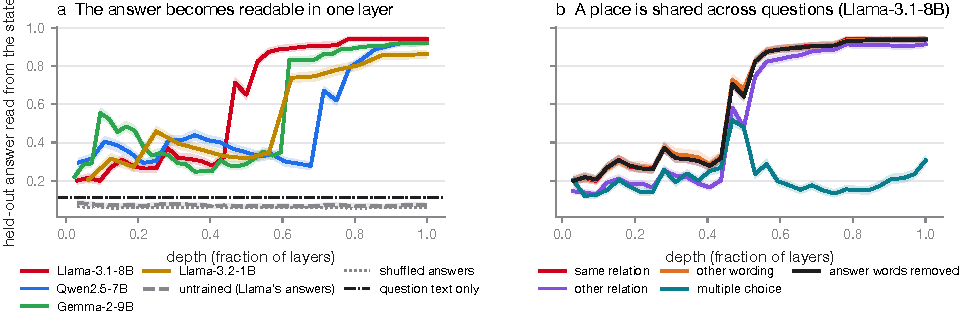
\includegraphics[width=\textwidth]{fig_decodability.pdf}
\caption{\textbf{Answers become readable at one depth, and what is read is a concept.} Held-out readability: the share of held-out questions whose nearest place (fitted on training subjects, same answer kind) is the answer the model gave; bands are 95\% intervals from resampling subjects. (a) All four models, with three controls: the same test on an untrained Llama-3.1-8B using the trained model's answers, labels shuffled between facts, and the question's text alone. (b) Llama-3.1-8B: places fitted on one relation and tested on the others (``other relation''); fitted on plain questions and tested on rewordings (``other wording''); with the answer words' output directions removed; and tested on the states of the multiple-choice version of the same questions.}
\label{fig:read}
\end{figure*}

The early plateau is not zero. Before the jump, 20--55\% of answers can be read, more than the shuffled control (\ShuffledLlama{}) and more than the question's text alone (\TextLlama{}--\TextQwen{}). We think this early signal reflects surface cues the model has already picked up from the subject's name, such as the language a name or title is in; we did not test this. Whatever its source, it does not grow with depth, and the jump goes far beyond it.

Three controls show that the structure is learned. An untrained Llama-3.1-8B, given the same prompts and grouped by the trained model's answers, never exceeds \UntrainedPeak{}. Shuffling answers between facts gives \ShuffledLlama{}--\ShuffledLlamaSmall{} at every layer. A classifier on the question's words alone reaches at most \TextQwen{}.

\paragraph{Tightness tells the same story.} Readability depends on a whitening of the state. The tightness ratio does not: it compares, in the model's own space, how far held-out questions sit from their place with how far places sit from each other. It falls 16- to 25-fold through the network (Figure~\ref{fig:tight}), and most of the fall happens at once. We fitted two shapes to the logarithm of each model's curve, a straight line (the same contraction at every layer, as seen in trained classifiers~\citep{he2022a}) and a single smooth step, and compared them by how well each predicts a left-out layer. The step wins in every model, by a factor of 5 to 24 in prediction error (Table~\ref{tab:models}).

\begin{figure}[t]
\centering
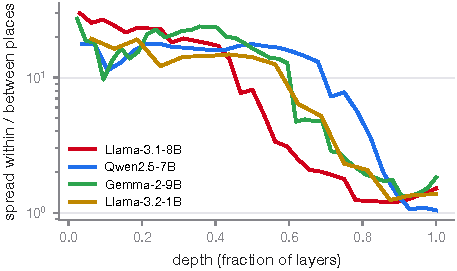
\includegraphics[width=\columnwidth]{fig_contraction.pdf}
\caption{\textbf{Tightness falls in a step.} Average squared distance of held-out questions from their place, divided by the spread of places, in each model's own space (log scale).}
\label{fig:tight}
\end{figure}

\begin{table}[t]
\centering
\footnotesize
\setlength{\tabcolsep}{2.6pt}
\begin{tabular}{@{}lcccc@{}}
\toprule
 & Llama 8B & Qwen 7B & Gemma 9B & Llama 1B \\
\midrule
Layers & \LayersLlama{} & \LayersQwen{} & \LayersGemma{} & \LayersLlamaSmall{} \\
Accuracy & \AccLlama{} & \AccQwen{} & \AccGemma{} & \AccLlamaSmall{} \\
Readable from (depth) & \OnsetLlama{} & \OnsetQwen{} & \OnsetGemma{} & \OnsetLlamaSmall{} \\
Peak readability & \PeakLlama{} & \PeakQwen{} & \PeakGemma{} & \PeakLlamaSmall{} \\
Error, step fit & \StepMseLlama{} & \StepMseQwen{} & \StepMseGemma{} & \StepMseLlamaSmall{} \\
Error, line fit & \LineMseLlama{} & \LineMseQwen{} & \LineMseGemma{} & \LineMseLlamaSmall{} \\
Other relation & \XRelLlama{} & \XRelQwen{} & \XRelGemma{} & \XRelLlamaSmall{} \\
Answer words removed & \NoWordsLlama{} & \NoWordsQwen{} & \NoWordsGemma{} & \NoWordsLlamaSmall{} \\
\bottomrule
\end{tabular}
\caption{\textbf{Per-model summary.} ``Readable from'': the layer, as a fraction of depth, at which readability first covers half the distance from chance to its peak, chosen on training subjects only. Step and line fits: mean squared error in predicting a left-out layer's log tightness. The last two rows are readability at 90\% of depth.}
\label{tab:models}
\end{table}

\section{A place is a concept, not a word}
\label{sec:concept}

If a place were only the model preparing to say a word, it would depend on how the question was asked and on the word's output direction. It depends on neither. A place fitted only on questions about people's citizenship finds the right country for questions about towns and films just as well: at 90\% of depth, \XRelLlama{} for Llama-3.1-8B, against \PeakLlama{} within the same relation (Figure~\ref{fig:read}b). Places fitted on plain questions work on casual or formal rewordings (\XWordLlama{}). And removing from the state every direction the output layer uses to write any of the 62 answer names, with the final normalisation's scaling taken into account, leaves readability unchanged (\NoWordsLlama{}); removing a random subspace of the same size does the same. The output layer does read these directions, so they are present, but the place does not depend on them.

The multiple-choice version of each question shows where the concept stops. When the options are listed and the model must answer with a letter, the content place is briefly readable from the multiple-choice state at the step (52\% in Llama-3.1-8B, against a shuffled level near 6\%), then fades to \ToMcqLlama{} as the state turns toward a letter. This matches the finding that models decide on the content of an option before binding it to its letter~\citep{wong2026when,wiegreffe2024answer}.

\section{Moving the state moves the answer}
\label{sec:steer}

Readability shows that the answer can be read from the place; it does not show that the model uses it. To test this we moved states. For a held-out question that the model answered wrongly, we added to its state, at one layer and at the last prompt position only, the difference between the right answer's place and the place of the answer it gave, and let the model answer again. As controls, we added a random direction of the same length, and we moved the state toward a third answer's place.

\begin{figure*}[t]
\centering
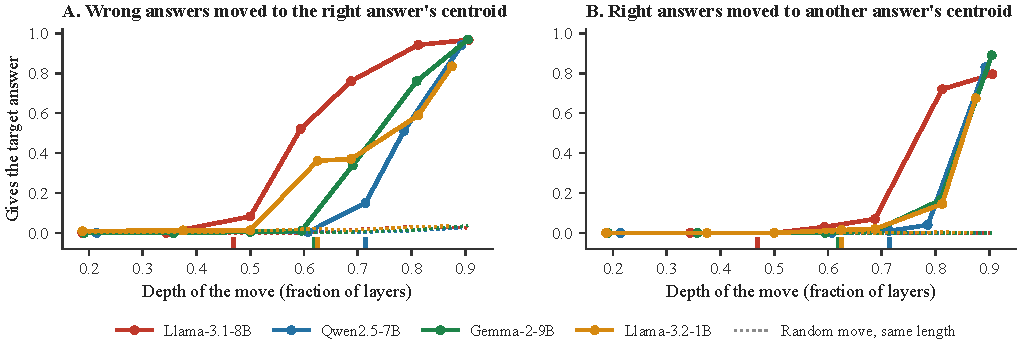
\includegraphics[width=\textwidth]{fig_steering.pdf}
\caption{\textbf{Moving a state into a place changes the answer, but only after the step.} (a) Wrong answers moved toward the right answer's place (solid) or by a random direction of the same length (dotted). (b) Right answers moved toward a different answer's place. The y-axis is the share of questions for which the model then gives the answer it was moved toward. Ticks under the axis mark the depth at which each model's answers become readable. Held-out questions; places from training subjects.}
\label{fig:steer}
\end{figure*}

The result follows the step (Figure~\ref{fig:steer}). Before a model's answers become readable, moves toward the right place do nothing: at 20\% of depth they correct \PushEarlyLlama{}--\PushEarlyLlamaSmall{} of wrong answers. After the step they work, and they work more the later they are made, reaching \PushGoldLlama{} (Llama-3.1-8B), \PushGoldQwen{} (Qwen2.5-7B), \PushGoldGemma{} (Gemma-2-9B) and \PushGoldLlamaSmall{} (Llama-3.2-1B) at about 90\% of depth. Random moves of the same length change \PushRandomLlama{}--\PushRandomGemma{} of these answers. The effect is not specific to the truth: moved toward a third answer's place, the model gives that answer \PushOtherQwen{}--\PushOtherGemma{} of the time, and right answers moved toward another place are given up for it \PushRightOtherLlamaSmall{}--\PushRightOtherGemma{} of the time. Each model follows the move only from the depth at which its own answers become readable, so the depth of the step measured by reading and the depth at which the model starts to act on the place agree.

Late moves are, in part, close to writing the answer directly, because late states are near the output. The informative parts of the experiment are the depth at which moves start to work, the failure of random moves, and the model's willingness to follow a move to any answer.

\section{Where wrong answers sit}
\label{sec:errors}

Because places are defined by what the model says, a wrong answer has a place too. At the depth where answers become readable, about half of the wrong answers that name a candidate sit nearest the place of the answer they gave (\AnatInGivenLlama{} for Llama-3.1-8B, \AnatInGivenQwen{} for Qwen2.5-7B), as confident mistakes, and \AnatInGoldLlama{} of all wrong answers sit nearest the right answer's place. This geometry carries information the output does not. For each wrong free-form answer we asked whether the model still picks the right option in the multiple-choice version (in more than half of the option orders it answered), and predicted this from the model's confidence in its reply, from the geometry of its state (distance to the right place, the right place's rank, and the margin to the nearest place), or from both, with five-fold cross-validation grouped by subject. Geometry predicts recognition better than confidence in every model (Figure~\ref{fig:errors}a): AUC \AucGeoLlama{} against \AucConfLlama{} for Llama-3.1-8B and \AucGeoGemma{} against \AucConfGemma{} for Gemma-2-9B, whose confidence carries no signal at all here. Adding geometry to confidence improves AUC in every model; the 95\% intervals for the gain, from resampling subjects, are \AucGainLoLlama{} to \AucGainHiLlama{} (Llama-3.1-8B), \AucGainLoQwen{} to \AucGainHiQwen{} (Qwen2.5-7B), \AucGainLoGemma{} to \AucGainHiGemma{} (Gemma-2-9B) and \AucGainLoLlamaSmall{} to \AucGainHiLlamaSmall{} (Llama-3.2-1B). The wrong answers studied number \ErrNLlama{}, \ErrNQwen{}, \ErrNGemma{} and \ErrNLlamaSmall{}.

\begin{figure*}[t]
\centering
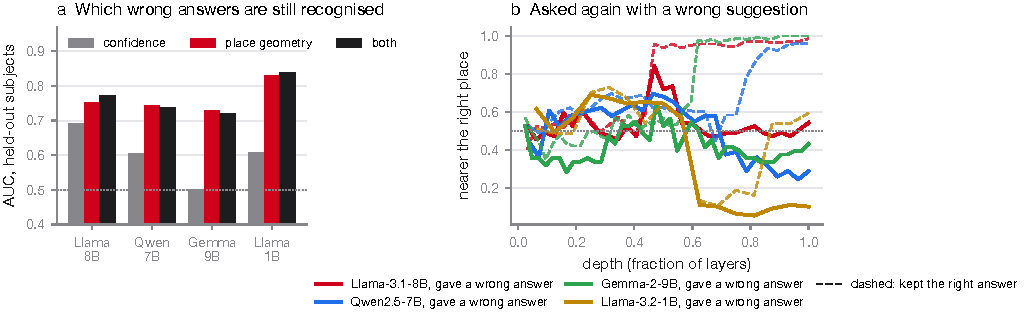
\includegraphics[width=\textwidth]{fig_errors.pdf}
\caption{\textbf{The geometry of a wrong answer says what the model still knows.} (a) Among wrong free-form answers on held-out subjects: how well the model's confidence in its reply, the geometry of its state at the step, or both, predict that it still picks the right option in multiple choice (AUC, five-fold cross-validation grouped by subject). (b) Questions answered correctly when asked plainly. With a user's wrong suggestion, those the model resisted (dashed) move to the right place and stay; those it was misled on (solid) first move toward the right place at the step, then away from it. Y-axis: share of states nearer the right answer's place than the suggested answer's place.}
\label{fig:errors}
\end{figure*}

The hint condition shows the same geometry in a case where we know what happened. For questions a model answers correctly when asked plainly, adding ``I'm fairly sure it's \dots'' with a wrong country sometimes changes the answer. Where the model resists, its state goes to the right place at the step and stays there (\HintResistEndLlama{} of states nearer the right place at the last layer of Llama-3.1-8B). Where the model is misled, the state first goes toward the right place too, with up to \HintPeakLlama{} of these states nearer it than the suggested place at about half depth, and then leaves it (\HintEndLlama{} at the last layer; \HintEndQwen{} in Qwen2.5-7B). Moving such a misled state back to the right place restores the right answer \PushMisledLlama{} of the time in Llama-3.1-8B. The model reached the answer it knew, and later layers replaced it.

\paragraph{Places hold beliefs.} Two models sometimes give different answers to the same question. If places reflected the question rather than the model's answer, both models' states would sit near the same place. They do not: in all \CrossModelPairs{} ordered pairs of models, on questions where the two disagree, each model's state is nearer its own answer's place than the other model's answer's place in \CrossModelMin{}--\CrossModelMax{} of cases.
